\documentclass[aspectratio=169]{beamer}


\usetheme[compress]{Drexel}

\author[S.~Lewis]{Sean Lewis}
\date[2018-24-07]{August 4, 2018}
\title[Progress Report]{\Huge Summer Research: \\ Hypervelocity Globular Cluster}
\institute{Drexel University}

\begin{document}

\begin{frame}
  \maketitle
\end{frame}

\section{HVGC-1}
\subsection{HVGC-1}

\begin{frame}
  {How BH phase affects ejection velocity}
  \begin{columns}
    \column{0.5\textwidth}
    \begin{itemize}
      \item Need to only consider phase-space that results in captured globular cluster. 
      \item If the GC does not achieve a distance of 120 pc after infall or takes too long to get there (makes more than one pass) final velocity is set to 0 km/s.
      \item Some energy from GC is transferred to BBH when it is captured.
    \end{itemize}
    \column{0.5\textwidth}
    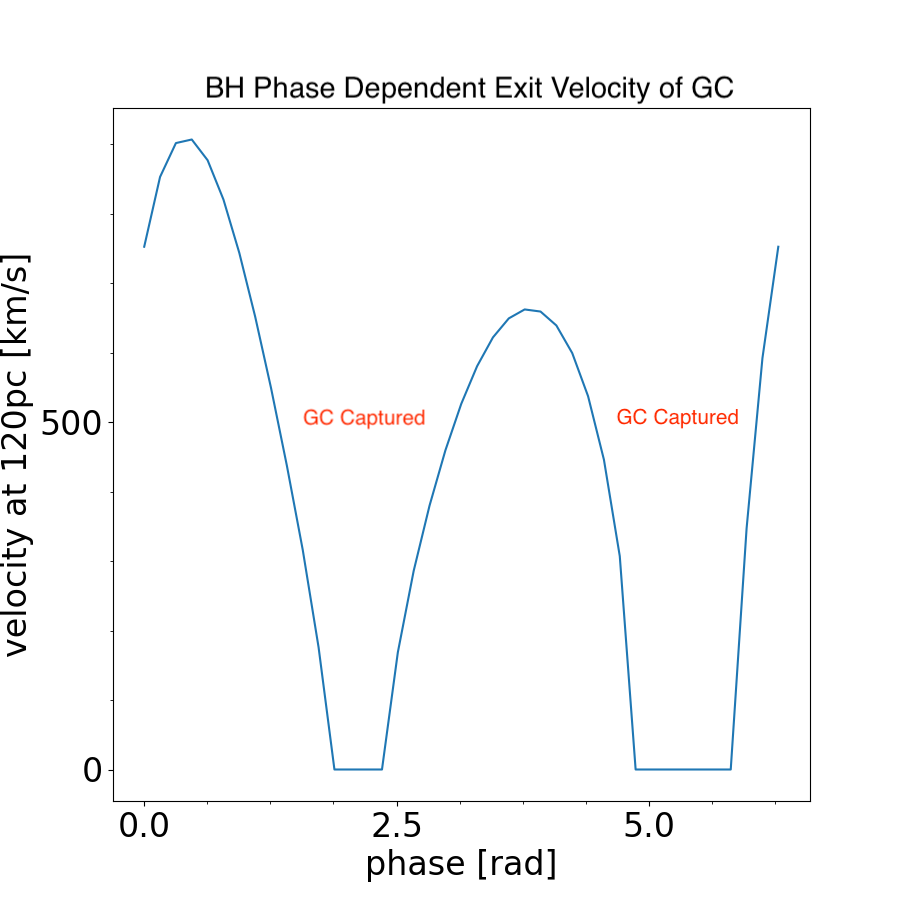
\includegraphics[width=6.4cm, height=6.4cm]{./Images/phase_loop_curated.png}
    \centering
  \end{columns}
\end{frame}

\begin{frame}
  {Energy Evolution of bound GC}
  \begin{columns}
    \column{0.5\textwidth}
    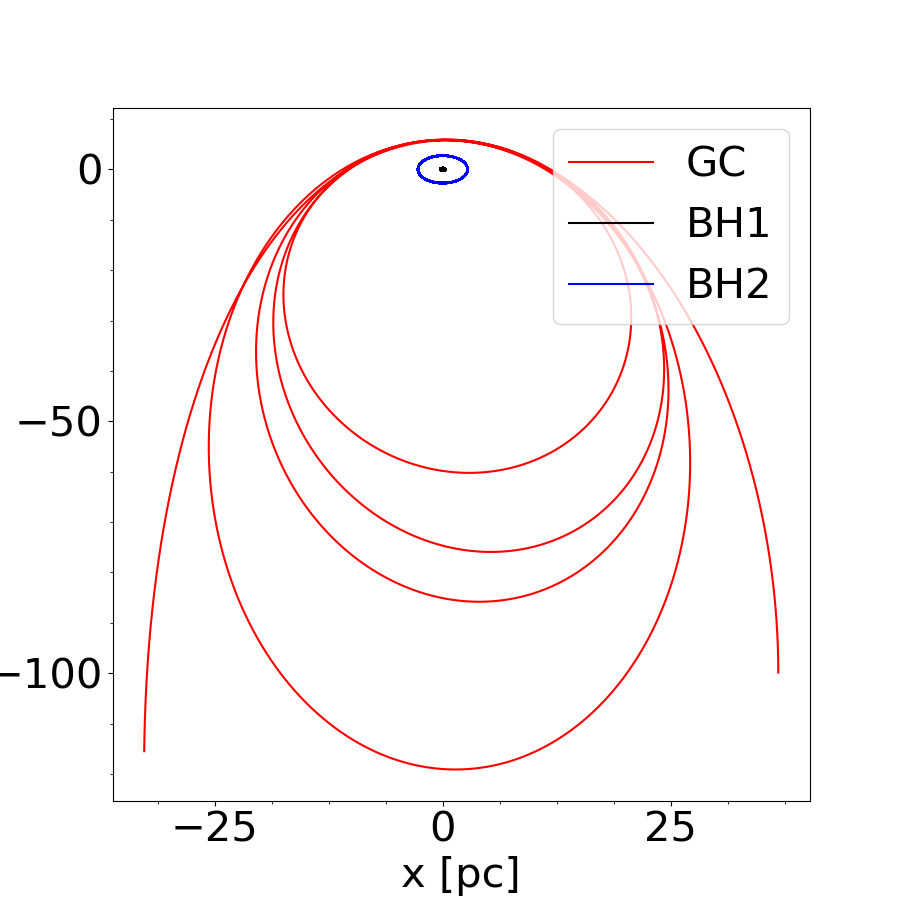
\includegraphics[width=6.4cm, height=6.4cm]{./Images/bound_track.png}
    \column{0.5\textwidth}
    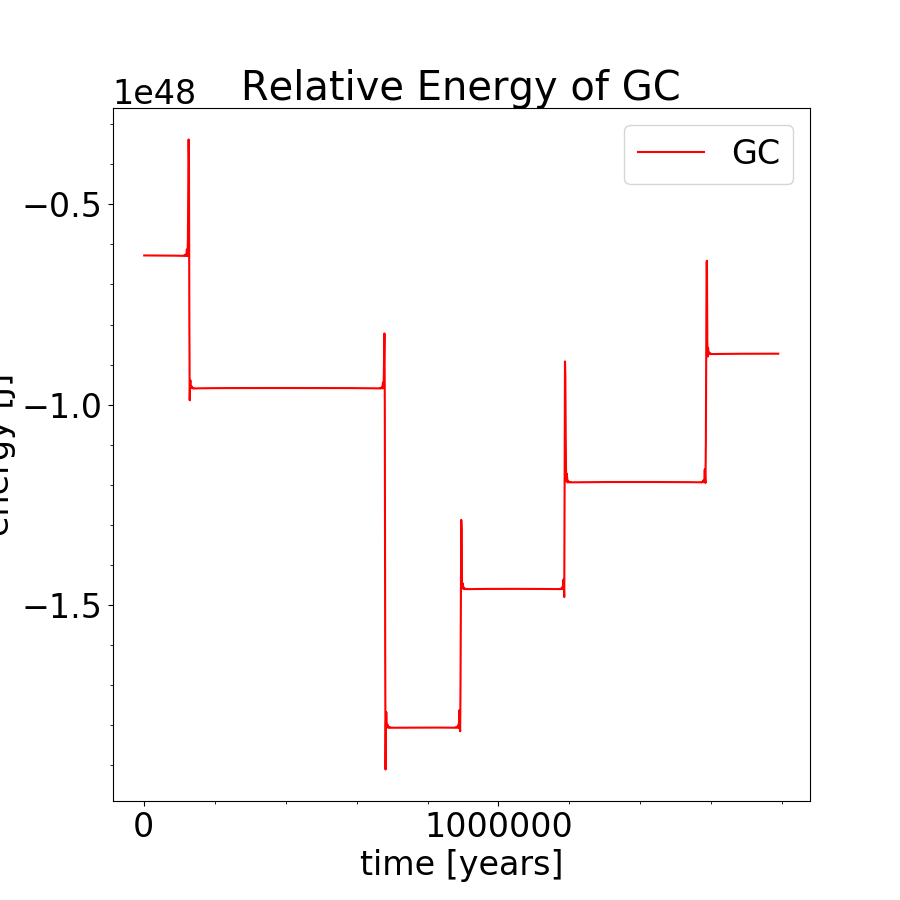
\includegraphics[width=6.4cm, height=6.4cm]{./Images/bound_energy.png}
  \end{columns}
\end{frame}

\begin{frame}
  {Energy Evolution of unbound GC}
  \begin{columns}
    \column{0.5\textwidth}
    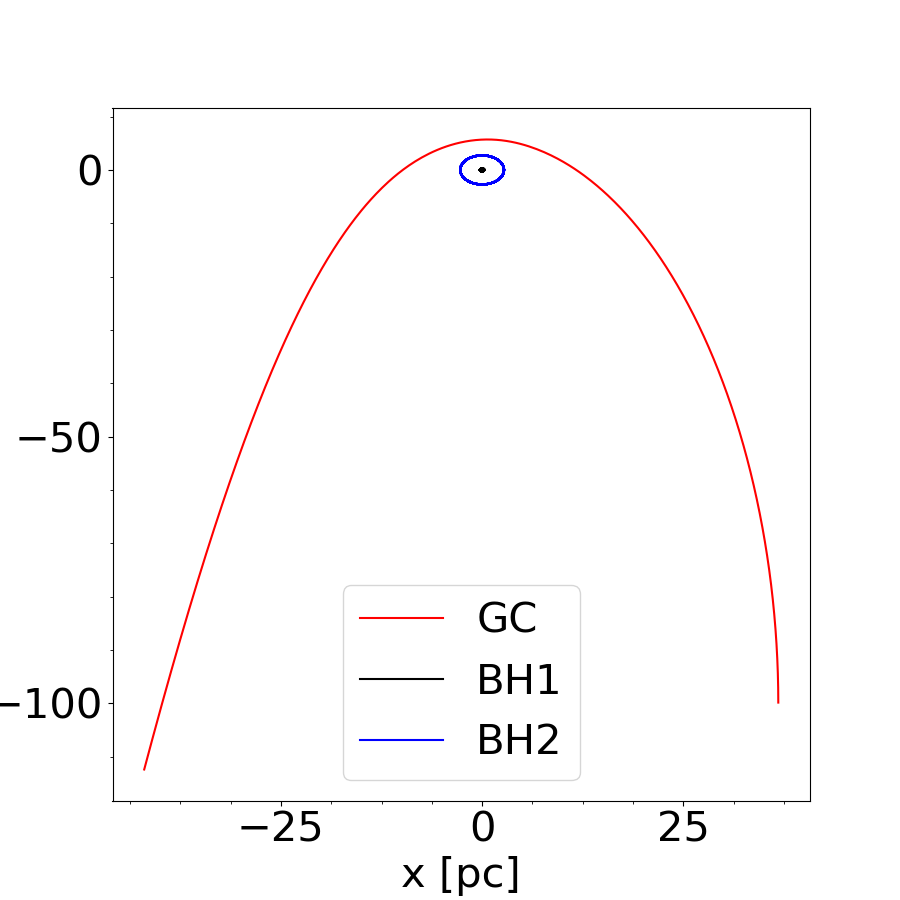
\includegraphics[width=6.4cm, height=6.4cm]{./Images/unbound_track.png}
    \column{0.5\textwidth}
    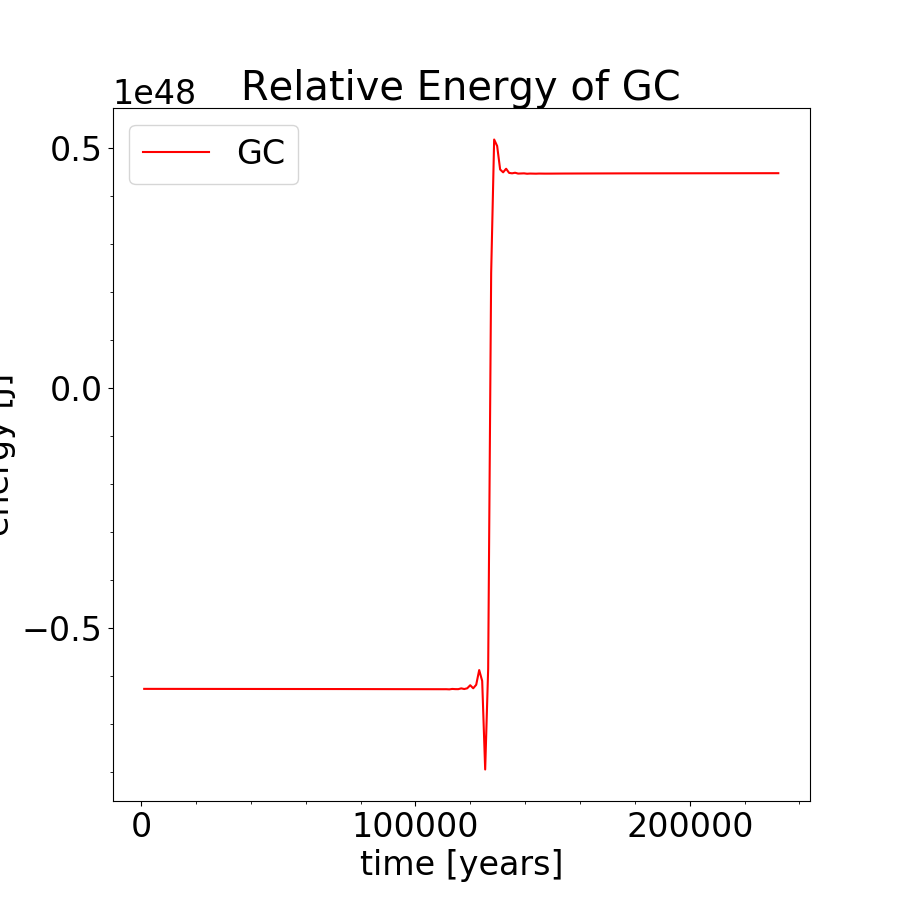
\includegraphics[width=6.4cm, height=6.4cm]{./Images/unbound_energy.png}
  \end{columns}
\end{frame}

\begin{frame}
  {Operational Parameters}
    \begin{itemize}
    \item Input: 
      \begin{itemize}
      \item Black holes: Mass ratio (1:100, 1:20, 1:10), separation (1.7, 3, 5) parsecs
      \item Globular Cluster: Closest approach (1.5, 2, 2.5) times BH separation
      \end{itemize}
    \item For each combination of operational parameters, cycle through initial black hole phases 0 to 2pi in steps of pi/20. ~1000 individual simulations, 7.5 min runtime.
    \item Outputs any velocity of ejected GC $>$ 1000 km/s, maximum tidal acceleration experienced, all operational params.
    
      (1108.74765364, 0.05, 1.7, 1.5, 0.785398163397)
    \item Interesting things: ZERO simulations with closest approach 2 or 2.5x BH separation and ZERO eith 0.01 BH mass ratio resulted in hypervelocity. 
    \end{itemize}
\end{frame}

\begin{frame}
  {Analysis to find optimum path}
  \begin{itemize}
    \item "Optimum path" meaning the interaction that results in highest ejection velocity and a low tidal acceleration.
    \item Want to find how far away from black hole binary the GC can get while still achieving a $>$ 1000 km/s velocity: 
    \begin{itemize}
      \item Repeat simulation set with new operational parameters. 
      \item Calculate tidal radius \& acceleration for each run.
    \end{itemize}
  \end{itemize}

\end{frame}

\backupbegin

\begin{frame}
  {}
  \begin{center}
    \Huge Backup Slides
  \end{center}
\end{frame}

\subsection{}
\begin{frame}
  {3:1 Mass ratio}
  \begin{columns}
    \column{0.5\textwidth}
    \begin{itemize}
      \item 2-3 pc pass from larger BH.
      \item Tidal radius of 0.3-0.4 pc
    \end{itemize}
    \column{0.6\textwidth}
    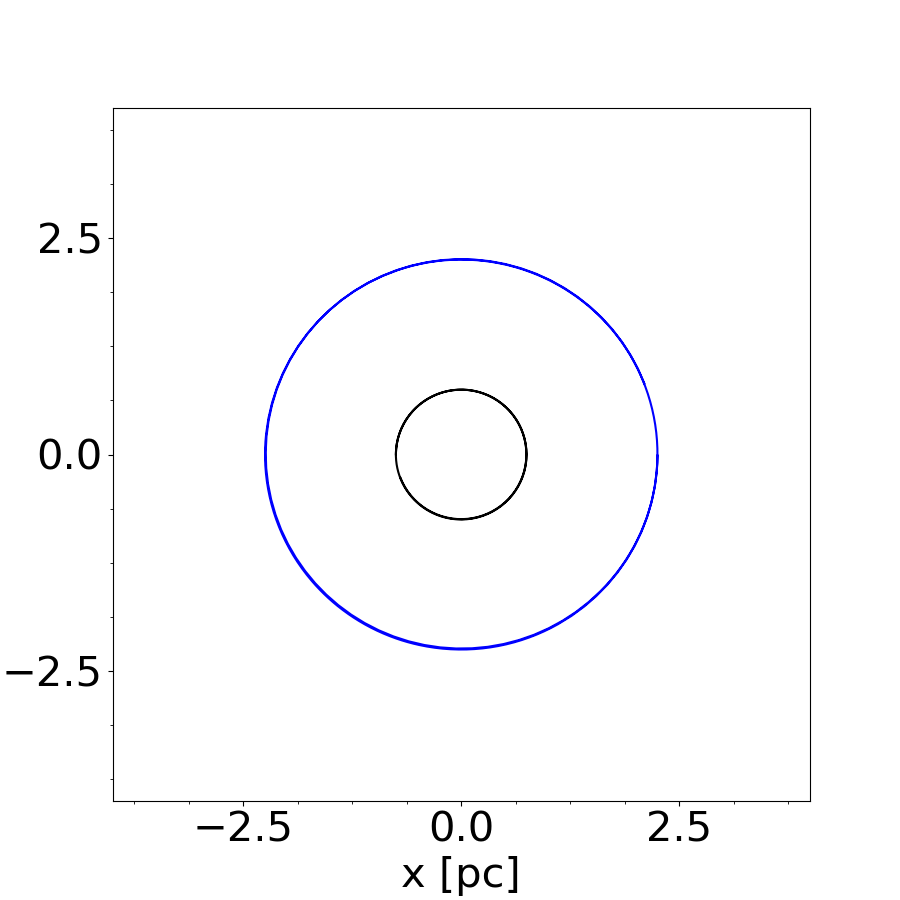
\includegraphics[width=6cm, height=6cm]{./Images/hvgc1_0333ratio.png}
    \centering
  \end{columns}
\end{frame}

\backupend
\end{document}